\subsection*{Code39}
%Herkunft und Nutzung
Code39 ist ein Strichcode, der 1974/75 von Intermec entwickelt wurde. Er kann max\-imal 43 alphanumerische Zeichen und Symbole verschlüsseln und wird verbreitet bei der Automobilherstellung, in der Elektrotechnik- und Elektronikindustrie genutzt.

%Aufbau
Er wird wie jeder andere Strichcode von einer Ruhezone umgeben, die die Auffindung des Codes vereinfacht. Sein Aufbau besteht dabei aus Gruppen zu neun Strichen~(5 schwarze, 4 weiße), wobei 3 davon dicker sind~(2 schwarze, 1 weißer), und zwischen den Gruppen wird ein weiterer weißer Strich eingefügt, der so dick wie die dünnen Striche ist. Dadurch können 40 Zeichen kodiert werden, wobei das 40igste leer gelassen wird. Als Anfangs- und Endsymbol werden dabei Sternchen kodiert. Später wurden zusätzlich noch 4 Sonderzeichen, die statt 2 schwarzer und einem weißen, 3 weiße Striche enthalten, hinzugefügt.

%Vorteile/Nachteile und zusätzliches
Vorteil des Code39 ist die hohe Zuverlässigkeit bei der Erkennung, da kaum Lesefehler vorkommen, Nachteil dagegen ist die Größe, da er 9 Striche für ein Zeichen/ Symbol nutzt. Er ist also die Beste Wahl, wenn kleine Gruppen von alphanumerischen Zeichen genutzt werden, wird aber zunehmend durch den Code 128 ersetzt.

\begin{figure}[H]
  \centering
  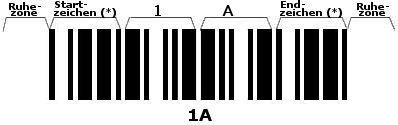
\includegraphics[height=3cm]{img/EAN13/code39-structure.jpg}
  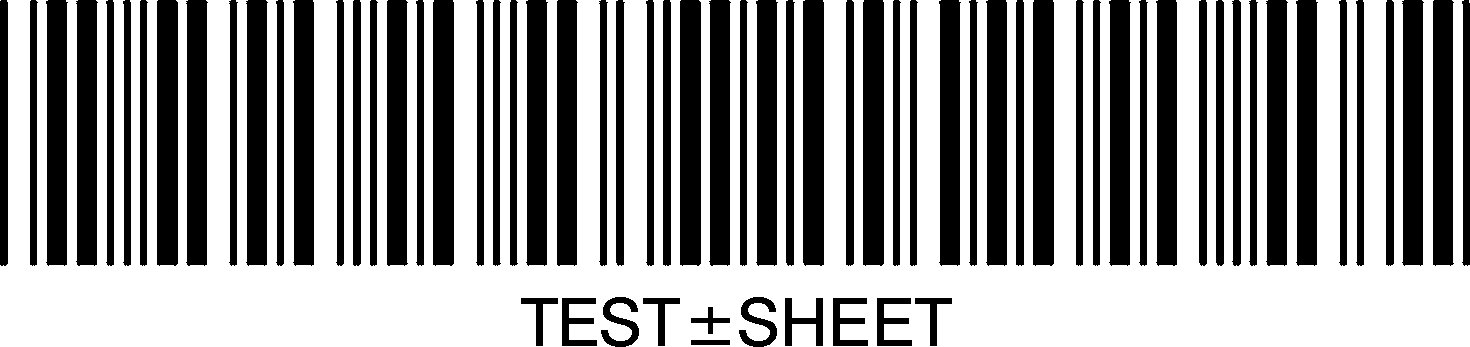
\includegraphics[height=3cm]{img/EAN13/code39.jpg}
  \caption{Der Aufbau des Code 39 und ein Beispielstrichcode.}
  \label{fig:code39}
\end{figure}

\todo{in Referenzen integrieren}
%Quelle:
%\url{http://aidc100.org/files/Allais-_David_Memoirs.pdf}
